% ============================================================
% ШИНЭ МОНГОЛ ТЕХНОЛОГИЙН КОЛЛЕЖ төгсөлтийн ажил
% Сувиллын бүртгэл мэдээллийн систем
% ============================================================

\documentclass[11pt, a4paper]{report}

% --- Фонт ба кодчилол (XeLaTeX ашиглана) ---
\usepackage{fontspec}
\setmainfont{Times New Roman}

% --- Хуудасны хэмжээ ---
\usepackage{geometry}
\geometry{
  left=2.5cm,
  right=2.0cm,
  top=2.0cm,
  bottom=2.0cm
}

% --- Мөрийн зай ---
\usepackage{setspace}
\singlespacing
\setlength{\parskip}{6pt}
\setlength{\parindent}{1.25cm}

% --- Монгол хэл ---
\usepackage{polyglossia}
\setmainlanguage{russian}  % Кирилл үсэг дэмжихэд ашигладаг
\newfontfamily\cyrillicfonttt{Courier New}
\addto\captionsrussian{%
  \renewcommand{\figurename}{Зураг}%
  \renewcommand{\tablename}{Хүснэгт}%
  \renewcommand{\contentsname}{Агуулга}%
  \renewcommand{\listfigurename}{Зургийн жагсаалт}%
  \renewcommand{\listtablename}{Хүснэгтийн жагсаалт}%
}

% --- Зураг, хүснэгт ---
\usepackage{graphicx}
\usepackage{float}
\usepackage{booktabs}
\usepackage{longtable}
\usepackage{array}
\usepackage{multirow}
\usepackage{amssymb}
\usepackage{xcolor}
\graphicspath{{figures/}}

% --- Гарчиг, хуудасны дугаар ---
\usepackage{hyperref}
\hypersetup{
  colorlinks=true,
  linkcolor=black,
  urlcolor=black,
  citecolor=black
}

% --- Ном зүй ---
\usepackage[backend=biber, style=numeric, sorting=none]{biblatex}
\addbibresource{references/refs.bib}

% URL хандсан огноо: "хандсан огноо: ЖЖЖЖ.СС.ӨӨ" формат
\DefineBibliographyStrings{russian}{
  urlseen = {хандсан огноо},
}
\renewbibmacro*{urldate}{%
  \iffieldundef{urlyear}{}%
  {%
    \printtext[parens]{%
      \bibstring{urlseen}\addcolon\addspace
      \thefield{urlyear}%
      \iffieldundef{urlmonth}{}{\adddot\mkdatezeros{\thefield{urlmonth}}}%
      \iffieldundef{urlday}{}{\adddot\mkdatezeros{\thefield{urlday}}}%
    }%
  }%
}

% --- Товчилсон үгсийн жагсаалт ---
\usepackage{acronym}

% --- Графикийн багц ---
\usepackage{tikz}
\usetikzlibrary{positioning, arrows.meta, shapes.geometric, shapes.multipart, calc}
\usepackage{pgfplots}
\pgfplotsset{compat=1.18}

% --- Зураг, хүснэгтийн жагсаалт ---
\usepackage[titles]{tocloft}

% --- Кодын блок ---
\usepackage{listings}
\lstset{
  basicstyle=\small\ttfamily,
  breaklines=true,
  frame=single,
  numbers=left,
  numberstyle=\tiny,
  keywordstyle=\bfseries,
}

% --- Байхгүй зургийн placeholder ---
\newcommand{\figplaceholder}[2][0.85]{%
  \IfFileExists{figures/#2.pdf}{%
    \includegraphics[width=#1\textwidth]{figures/#2}%
  }{\IfFileExists{figures/#2.png}{%
    \includegraphics[width=#1\textwidth]{figures/#2}%
  }{\IfFileExists{figures/#2.svg}{%
    \includegraphics[width=#1\textwidth]{figures/#2}%
  }{%
    \fbox{\parbox{#1\textwidth}{\centering\vspace{1.8cm}\textit{[Зураг оруулах: #2]}\vspace{1.8cm}}}%
  }}}%
}

% --- Бүлгийн гарчгийн формат ---
\usepackage{titlesec}
\titleformat{\chapter}[block]
  {\normalfont\Large\bfseries}
  {\thechapter}{1em}{}
\titlespacing*{\chapter}{0pt}{0pt}{12pt}
\titleformat{\section}[block]
  {\normalfont\large\bfseries}
  {\thesection}{1em}{}
\titlespacing*{\section}{0pt}{12pt}{6pt}
\titleformat{\subsection}[block]
  {\normalfont\normalsize\bfseries}
  {\thesubsection}{1em}{}
\titlespacing*{\subsection}{0pt}{10pt}{4pt}

% ============================================================
\begin{document}

\pagenumbering{roman}   
\setcounter{page}{0}   

% --- НҮҮР ХУУДАС ---
\begin{titlepage}
    \centering
    
    % 1. Толгой хэсэг (Лого + Сургуулийн нэр)
    \begin{minipage}{0.15\textwidth}
        
\includegraphics[width=\textwidth]{figures/Logo.png}
    \end{minipage}
    \begin{minipage}{0.8\textwidth}
        \centering
        \textbf{\large ШИНЭ МОНГОЛ ТЕХНОЛОГИЙН КОЛЛЕЖ}\\[0.1cm]
        \textbf{\large КОМПЬЮТЕРЫН УХААНЫ ТЭНХИМ}
    \end{minipage}

    \vspace{3cm}

    % 2. Оюутны мэдээлэл 
    \begin{flushright}
        \begin{tabular}{r}
            Оюутны код: s21c118b \\ [0.2cm]
            Оюутны нэр: Бямбасүрэн Зөнсод
        \end{tabular}
    \end{flushright}

    \vspace{4cm}

    % 3. Төслийн гарчиг
    {\Large \textbf{\MakeUppercase{Сувиллын бүртгэл мэдээллийн систем}}}\\[0.4cm]
    {\normalsize /ДЭД БАКАЛАВРЫН ТӨГСӨЛТИЙН СУДАЛГААНЫ АЖИЛ/}

    \vspace{2cm} % Доод талын удирдагчийн хэсгийг доош түлхэнэ

    % 4. Удирдагч болон Гүйцэтгэгч (Зүүн болон баруун талд)
    \begin{minipage}{0.95\textwidth}
        \begin{tabular*}{\textwidth}{@{\extracolsep{\fill}}l r@{}}
            Удирдсан багш: & /Магистр: Б.Батчулуун/ \\[0.4cm]
            Гүйцэтгэсэн оюутан: & /Б.Зөнсод s21c118b/
        \end{tabular*}
    \end{minipage}

    \vfill % Доод хот, он хүртэлх зай

    % 5. Доод хэсэг
    {\normalsize Улаанбаатар хот\\2026 он}
\end{titlepage}
\newpage % Шинэ хуудас эхлүүлэх

% --- ХОЁР ДАХЬ НҮҮР ХУУДАС (INTERNAL TITLE PAGE) ---
\begin{titlepage}
    \centering
    
    % 1. Сургуулийн нэр
    \textbf{\large \MakeUppercase{Шинэ Монгол Технологийн Коллеж}}\\[0.2cm]
    \textbf{\large \MakeUppercase{Компьютерын ухааны тэнхим}}

    \vfill % Зай авах

    % 2. Ажлын төрөл болон Гарчиг
    {\normalsize Дэд бакалаврын төгсөлтийн судалгааны ажил}\\[0.6cm]
    {\Large \textbf{\MakeUppercase{Сувиллын бүртгэл мэдээллийн систем}}}\\[0.4cm]
    \vspace{2cm} % Зай авах

    % 3. Гүйцэтгэгч болон Удирдагч (Голлуулсан)
    {\large \textbf{Гүйцэтгэгч:}} Б.Зөнсод\\[0.5cm]
    {\large \textbf{Удирдагч:}} Б.Батчулуун, Магистр

    \vfill % Зай авах

    % 4. Доод хэсэг
    {\normalsize Улаанбаатар хот\\2026 он}

\end{titlepage}
\newpage
\setcounter{page}{1}    % ← Хураангуй = i
% --- ХУРААНГУЙ ХУУДАС (ABSTRACT) ---
\begin{center}
    \textbf{\large \MakeUppercase{Сувиллын бүртгэл мэдээллийн систем}}\\[0.2cm]
\end{center}

\vspace{0.5cm}

\begin{flushright}
    \begin{spacing}{1.2}
        {\normalsize Компьютерын ухааны тэнхим}\\
        {\normalsize Оюутан: Б.Зөнсод s21c118b}\\
        {\normalsize Удирдсан багш: Б.Батчулуун, Магистр}
    \end{spacing}
\end{flushright}

\vspace{0.5cm}

\begin{center}
    \textbf{\MakeUppercase{Хураангуй}}
\end{center}

\vspace{0.3cm}

% --- Хураангуйн эх бие ---
Өнөөдрийн байдлаар Өвөрхангай аймгийн Хужирт сумын сувиллуудын ихэнх нь үйлчлүүлэгч бүртгэх, өрөө захиалах үйл явцыг утсаар ярьж захиалдаг уламжлалт аргаар хэрэгжүүлж байна. 
 Захиалга баталгаажуулах, ирц хянах, тайлан гаргах зэрэг ажлуудыг цаасан бүртгэл болон хүний гараар гүйцэтгэх нь мэдээллийн алдагдал, захиалгын давхардал, ажилтны ачаалал нэмэгдэх зэрэг үйл ажиллагааны хүндрэлийг үүсгэж байна.

Иймд энэхүү судалгааны ажлын хүрээнд сувиллын захиалга үүсгэх, үйлчлүүлэгчийн бүртгэл хөтлөх, ажилтны хяналт болон захиргааны тайлан нэгтгэх боломж бүхий веб суурьтай нэгдсэн системийг хөгжүүлэхийг зорив. Тус систем нь сувиллын захиалгын үйл явцыг цахимжуулж, амрагч, ажилтан, администраторын хэрэгцээг нэг платформд нэгтгэсэн удирдлагын орчныг бий болгосноор үйлчилгээний чанар болон байгууллагын үйл ажиллагааны үр ашгийг дээшлүүлэхэд чиглэнэ.

\vspace{1cm}

\noindent \textbf{Түлхүүр үг:} Сувиллын бүртгэл, Захиалгын систем, Вэб хөгжүүлэлт, Өгөгдлийн сан.

% --- 4. Гарчиг ---
\newpage
\phantomsection
\addcontentsline{toc}{chapter}{Гарчиг}

\noindent\textbf{Гарчиг}
\vspace{0.5cm}
\newcommand{\tocchapter}[2]{%
  \noindent\textbf{#1}\dotfill\textbf{#2}\par\vspace{6pt}%
}
\newcommand{\tocchapternd}[2]{%
  \noindent\textbf{#1}\hfill\textbf{#2}\par\vspace{6pt}%
}
\newcommand{\tocnumchapter}[3]{%
  \noindent\textbf{#1\quad #2}\dotfill\textbf{#3}\par\vspace{6pt}%
}
\newcommand{\tocsection}[3]{%
  \noindent\hspace{1em}#1\quad #2\dotfill #3\par\vspace{3pt}%
}
\newcommand{\tocsubsection}[3]{%
  \noindent\hspace{2.5em}#1\quad #2\dotfill #3\par\vspace{2pt}%
}

\tocchapternd{Хураангуй}{i}
\tocchapternd{Гарчиг}{ii}
\tocchapternd{Товчилсон үгсийн жагсаалт}{iv}
\tocchapternd{Хүснэгтийн жагсаалт}{v}
\tocchapternd{Зургийн жагсаалт}{vi}

\vspace{6pt}

% --- Бүлэг 1 ---
\tocnumchapter{1}{Удиртгал}{1}
\tocsection{1.1}{Үндэслэл, ач холбогдол}{x}
\tocsection{1.2}{Судалгааны ажлын зорилго}{x}
\tocsection{1.3}{Судалгааны ажлын зорилтууд}{x}

% --- Бүлэг 2 ---
\tocnumchapter{2}{Онолын хэсэг}{x}
\tocsection{2.1}{Өнөөгийн байдлын судалгаа}{x}
\tocsubsection{2.1.1}{Client-Server загвар}{x}
\tocsubsection{2.1.2}{REST API зарчим}{x}
\tocsection{2.2}{Технологийн Stack сонголт}{x}
\tocsubsection{2.2.1}{Next.js}{x}
\tocsubsection{2.2.2}{Prisma ORM}{x}
\tocsubsection{2.2.3}{PostgreSQL}{x}
\tocsubsection{2.2.4}{Supabase}{x}
\tocsection{2.3}{Өгөгдлийн сан ба Аюулгүй байдал}{x}
\tocsubsection{2.3.1}{Relational model}{x}
\tocsubsection{2.3.2}{JWT - JSON Web Token}{x}
\tocsubsection{2.3.3}{NextAuth.js}{x}

% --- Бүлэг 3 ---
\tocnumchapter{3}{Судалгааны арга зүй}{x}
\tocsection{3.1}{Системийн үйл ажиллагааны тухай дэлгэрэнгүй}{x}
\tocsubsection{3.1.1}{Системийн ерөнхий бүтэц}{x}
\tocsubsection{3.1.2}{Системийн үндсэн урсгал}{x}
\tocsection{3.2}{Системийн хэрэглэгчид}{x}
\tocsection{3.3}{Функционал шаардлага}{x}
\tocsection{3.4}{Функционал бус шаардлага}{x}
\tocsection{3.5}{Юзкейс диаграммууд}{x}
\tocsubsection{3.5.1}{Үйлчлүүлэгчийн юзкейс диаграмм}{x}
\tocsubsection{3.5.2}{Ажилтан болон Админы юзкейс диаграмм}{x}
\tocsection{3.6}{Дарааллын диаграммууд}{x}
\tocsubsection{3.6.1}{Бүртгэл ба нэвтрэлтийн дараалал}{x}
\tocsubsection{3.6.2}{Захиалга үүсгэх дараалал}{x}
\tocsubsection{3.6.3}{Захиалга баталгаажуулах дараалал}{x}
\tocsection{3.7}{Өгөгдлийн сангийн ерөнхий загвар}{x}
\tocsubsection{3.7.1}{Үндсэн хүснэгтүүд ба харилцаа холбоо}{x}
\tocsubsection{3.7.2}{Хүснэгтүүдийн тайлбар}{x}

% --- Бүлэг 4 ---
\tocnumchapter{4}{Судалгааны үр дүн, дүгнэлт}{x}

\vspace{6pt}

\tocchapter{Ном зүй}{x}
\tocchapter{Товчлол}{x}
\tocchapter{Хавсралт}{x}

% --- 5. ТОВЧИЛСОН ҮГСИЙН ЖАГСААЛТ ---
% --- ТОВЧИЛСОН ҮГСИЙН ЖАГСААЛТ ---
\newpage
\chapter*{Товчилсон үгсийн жагсаалт}
\addcontentsline{toc}{chapter}{Товчилсон үгсийн жагсаалт}
\begin{acronym}
  \acro{СҮУЗС}{Сувиллын үйлчилгээний удирдлага, захиалгын систем}
  \acro{API}{Application Programming Interface — програмын холбоосын интерфэйс}
  \acro{DB}{Database — өгөгдлийн сан}
  \acro{UI/UX}{User Interface / User Experience — хэрэглэгчийн интерфэйс / туршлага}
  \acro{JWT}{JSON Web Token — токен суурьтай нэвтрэлт баталгаажуулах арга}
  \acro{RLS}{Row-Level Security — мөр түвшний хандалтын хяналт}
  \acro{SUS}{System Usability Scale — системийн ашиглах чадварын хэмжүүр}
  \acro{ORM}{Object-Relational Mapping — объект-харилцааны зурагчлал}
  \acro{REST}{Representational State Transfer — төлөвийн дамжуулалтын архитектур}
  % --- Арга зүйн нэр томьёо ---
  \acro{applied research}{практик судалгаа}
  \acro{iterative development}{давтамжтай хөгжүүлэлт}
  \acro{waterfall}{дараалсан хөгжүүлэлтийн загвар}
  \acro{working increment}{ажиллагаатай хувилбар}
  \acro{concurrency}{зэрэг хандалт}
  \acro{usability}{ашиглах чадвар}
  \acro{full-stack}{бүрэн хэмжээний веб хөгжүүлэлт}
\end{acronym}


% --- 6. ХҮСНЭГТИЙН ЖАГСААЛТ ---
\newpage
\chapter*{Хүснэгтийн жагсаалт}
\addcontentsline{toc}{chapter}{Хүснэгтийн жагсаалт}
\begingroup
\renewcommand{\clearpage}{} 
\renewcommand{\chapter}[2]{} 
\listoftables
\endgroup

% --- 7. ЗУРГИЙН ЖАГСААЛТ ---
\newpage
\chapter*{Зургийн жагсаалт}
\addcontentsline{toc}{chapter}{Зургийн жагсаалт}
\begingroup
\renewcommand{\clearpage}{} 
\renewcommand{\chapter}[2]{} 
\listoffigures
\endgroup

% --- 7. АЖЛЫН ТӨЛӨВЛӨГӨӨ ---
\newpage
\addcontentsline{toc}{chapter}{Ажлын төлөвлөгөө}

\vspace*{0.5cm}
\noindent\textbf{\large Ажлын төлөвлөгөө}

\vspace{15pt}
\noindent\textbf{Оюутны нэр:} Б.Зөнсод \hfill \textbf{Удирдагч багшийн нэр:} Б.Батчулуун\\[10pt]
\noindent\textbf{Судалгааны ажлын сэдэв:} Сувиллын бүртгэл мэдээллийн систем

\vspace{10pt}
\begin{center}
\renewcommand{\arraystretch}{1.3}
\begin{longtable}{|c|c|p{10.5cm}|c|}
\hline
\textbf{Сар} & \textbf{Долоо хоног} & \textbf{Төлөвлөгөө} & \textbf{Гүйцэтгэл} \\
\hline
\endfirsthead
\hline
\textbf{Сар} & \textbf{Долоо хоног} & \textbf{Төлөвлөгөө} & \textbf{Гүйцэтгэл} \\
\hline
\endhead
\multirow{4}{*}{10 сар} & 1 & & $\checkmark$ \\ \cline{2-4}
& 2 & Веб системийн онол, технологийн судалгаа (Next.js, Prisma, PostgreSQL гэх мэт) & $\checkmark$ \\ \cline{2-4}
& 3 & Сувиллын захиалга авах урсгалыг ойлгох, тулгамдаж буй гол асуудлыг тодорхойлох & $\checkmark$ \\ \cline{2-4}
& 4 & Системийн шаардлагын шинжилгээ гаргах & $\checkmark$ \\
\hline
\multirow{4}{*}{11 сар} & 1 & Системийн архитектур ба өгөгдлийн сангийн загвар боловсруулах & $\checkmark$ \\ \cline{2-4}
& 2 & Front-end хэсгийн бүтцийг боловсруулах (Next.js, TailwindCSS) & $\checkmark$ \\ \cline{2-4}
& 3 & Back-end API ботыг tRPC ба Prisma ашиглан хөгжүүлж эхлэх & $\checkmark$ \\ \cline{2-4}
& 4 & PostgreSQL өгөгдлийн сан үүсгэх, API холболт хийх & $\checkmark$ \\
\hline
\multirow{4}{*}{12 сар} & 1 & \textcolor{red}{ТСА Үзлэг 1} & $\checkmark$ \\ \cline{2-4}
& 2 & Front-end болон Back-end интеграц, анхны туршилт хийх & $\checkmark$ \\ \cline{2-4}
& 3 & Системийн анхны хувилбарыг турших, алдаа засварлах & $\checkmark$ \\ \cline{2-4}
& 4 & Хэрэглэгчийн болон админ хэсгийн интерфейс сайжруулах & $\checkmark$ \\
\hline
\multirow{4}{*}{1 сар} & 1 & Функциональ туршилт хийх, өгөгдөл нэмэх & $\checkmark$ \\ \cline{2-4}
& 2 & Туршилтын үр дүнг нэгтгэж, сайжруулалт хийх & $\checkmark$ \\ \cline{2-4}
& 3 & Системийн гүйцэтгэл ба найдвартай байдлын шалгалт & $\checkmark$ \\ \cline{2-4}
& 4 & Системийг үүлэн (Cloud) орчинд байршуулж турших & $\checkmark$ \\
\hline
\multirow{4}{*}{2 сар} & 1 & Тест хэрэглэгчээр туршилт хийх, алдаа илрүүлэх & $\checkmark$ \\ \cline{2-4}
& 2 & Тайлан бичих, үр дүнгийн дүгнэлт боловсруулах & $\checkmark$ \\ \cline{2-4}
& 3 & Тайланг сайжруулах, багшийн зөвлөмж тусгах & $\checkmark$ \\ \cline{2-4}
& 4 & Туршилтын үр дүнг нэгтгэх, диаграмм, хүснэгт боловсруулах & $\checkmark$ \\
\hline
\multirow{4}{*}{3 сар} & 1 & \textcolor{red}{ТСА Үзлэг 2} & $\square$ \\ \cline{2-4}
& 2 & Эцсийн системийн хувилбар гаргах & $\square$ \\ \cline{2-4}
& 3 & Хамгаалалтын материал бэлтгэх & $\square$ \\ \cline{2-4}
& 4 & Удирдагч багшийн зөвлөгөөний дагуу сайжруулалт & $\square$ \\
\hline
\multirow{4}{*}{4 сар} & 1 & Удирдагч багшийн зөвлөгөөний дагуу сайжруулалт & $\square$ \\ \cline{2-4}
& 2 & Удирдагч багшийн зөвлөгөөний дагуу сайжруулалт & $\square$ \\ \cline{2-4}
& 3 & Удирдагч багшийн зөвлөгөөний дагуу сайжруулалт & $\square$ \\ \cline{2-4}
& 4 & \textcolor{red}{ТСА урьдчилсан хамгаалалт} & $\square$ \\
\hline
\multirow{4}{*}{5 сар} & 1 & & $\square$ \\ \cline{2-4}
& 2 & & $\square$ \\ \cline{2-4}
& 3 & & $\square$ \\ \cline{2-4}
& 4 & \textcolor{red}{ТСА үндсэн хамгаалалт} & $\square$ \\
\hline
\end{longtable}
\end{center}

\vspace{0.8cm}
\noindent
\begin{minipage}{0.5\textwidth}
Удирдагч багш \\
Гүйцэтгэсэн оюутан 
\end{minipage}%
\begin{minipage}{0.5\textwidth}
\raggedleft
/Б.Батчулуун, магистр/ \\
/s21c118b, Б.Зөнсод/
\end{minipage}


% --- ҮНДСЭН ХЭСЭГ (ARABIC NUMERALS) ---
\newpage
\pagenumbering{arabic}

% Бүлэг 1
\chapter{УДИРТГАЛ}

\section{Үндэслэл, ач холбогдол}

Хөдөө орон нутагт рашаан, шавар эмчилгээний үйл ажиллагаа явуулдаг 20 гаруй сувиллууд байдаг. Тэдгээр сувиллуудын өнөөгийн захиалга авах үйл явц дараах алхмуудаас бүрдэж байна. Үүнд:

\begin{itemize}
    \item Үйлчлүүлэгч тухайн сувиллын хүлээн авах утас руу залгана.
    \item Хүлээн авах ажилтан захиалгын мэдээллийг цаасан дээр гараар тэмдэглэнэ.
    \item Хэвтэн эмчлүүлэх захиалга товлосон өдөр дөхөх үед, ажилтан үйлчлүүлэгч рүү эргэж залган урьдчилгаа төлбөр авах, ирэх эсэхийг дахин баталгаажуулна.
\end{itemize}

Энэ урсгал нь удаан хугацаанд хэрэглэгдэж ирсэн ч дараах асуудлуудыг үүсгэж байна:

\begin{itemize}
    \item Үйлчлүүлэгч захиалгаа урьдчилан мэдэгдэлгүй цуцлах, эсвэл хоорондын ойлголцлын зөрөөнөөс шалтгаалж огноо, хүмүүсийн тоо зэрэг алдаа гарах.
    \item Хүлээн авах ажилтны гар тэмдэглэл алдагдах, гээх зэрэг хүний хүчин зүйлээс шалтгаалсан эрсдэл.
    \item Утасны ачааллаас шалтгаалан шуурхай хариу өгөх боломжгүй байх.
    \item Тайлан тооцоог нарийвчлалтай гаргахад хүндрэлтэй.
\end{itemize}

Иймээс хэзээ ч, хаанаас ч вэбээр захиалга өгөх боломжтой амрагчийн захиалгын системийг нэвтрүүлэх хэрэгцээ бодитойгоор бий болсон гэж үзсэн. Энэхүү судалгааны ажлын үр дүн нь тухайн нэг байгууллага төдийгүй ижил төрлийн бусад сувиллын байгууллагуудад ч хэвшүүлэх, ашиглах боломжтой жишиг загвар болох ач холбогдолтой билээ.

\section{Судалгааны ажлын зорилго}

Энэхүү судалгааны ажлын ерөнхий зорилго нь Өвөрхангай аймгийн Хужирт сумын сувиллын онцлогт тохируулсан амрагчийн захиалгын бүртгэл болон захиалгыг хянах админ системийг вэб хэлбэрээр боловсруулж, захиалга авах үйл явцыг илүү үр ашигтай, алдаа багатай, ашиглахад хялбар болгох юм.

\section{Судалгааны ажлын зорилтууд}

Дээрх зорилгыг хэрэгжүүлэхийн тулд дараах зорилтуудыг дэвшүүлж байна.

\begin{enumerate}
    \item Хүлээн авах ажилтан болон удирдлагад тулгарч буй асуудал, одоогийн захиалгын урсгал, түүнээс үүдэлтэй хохирол, эрсдэлийг тодорхойлох.
    \item Сувиллын үйлчлүүлэгч, ажилтнуудын хэрэгцээнд нийцсэн вэб суурьтай захиалгын системийн шаардлага, архитектур, интерфейсийг тодорхойлох.
    \item Захиалга авах, баталгаажуулах, админаар хянах, тайлан, статистик гаргах боломж бүхий вэб системийн frontend болон backend хэсгийг хөгжүүлж, PostgreSQL өгөгдлийн сантай уялдуулан туршилтын хувилбарыг програмчлах.
    \item Хөгжүүлсэн системийг cloud server (AWS) орчинд байршуулж, жинхэнэ эсвэл туршилтын хэрэглэгчдээр ашиглуулан туршилт, үнэлгээ хийж, санал хүсэлтийн дагуу сайжруулалт хийх.
\end{enumerate}
\section{Судалгааны асуулт ба хэмжигдэх шалгуур}

Судалгааны ажлын зорилтуудыг хэмжихүйц шалгууруудтай холбохын тулд дараах судалгааны асуултуудыг тодорхойлов. Асуулт бүрийн хариуг баруун баганад буй тодорхой хэмжүүрээр үнэлнэ.

\begin{table}[H]
\centering
\caption{Судалгааны асуулт ба үнэлгээний шалгуур үзүүлэлтүүд}
\label{tab:research-questions}
\begin{tabular}{|c|p{5.5cm}|p{6cm}|}
\hline
\textbf{RQ} & \textbf{Судалгааны асуулт} & \textbf{Хэмжих шалгуур үзүүлэлт} \\
\hline
RQ1 & Вэб суурьтай захиалгын систем нь цаасан бүртгэл, утсаар захиалга авах процесстой харьцуулахад захиалга боловсруулах хугацааг бууруулж чадах уу? & Нэг захиалга боловсруулах дундаж хугацаа (секунд), мэдээлэл хайх хугацаа, тайлан гаргах хугацааны харьцуулалт \\
\hline
RQ2 & Систем нь давхар захиалга (double-booking), огнооны зөрөө зэрэг хүний алдаанаас үүдэлтэй асуудлуудыг арилгаж чадах уу? & Зэрэг хандалтын туршилтаар илэрсэн давхар захиалгын тоо, pessimistic locking-ийн амжилтын хувь \\
\hline
RQ3 & Системийн ашиглах чадвар (usability) хүлээн зөвшөөрөгдөхүйц түвшинд байх уу? & System Usability Scale (SUS) оноо 68-аас дээш байх, даалгавар гүйцэтгэх амжилтын хувь \\
\hline
\end{tabular}
\end{table}

% Бүлэг 2
\chapter{Онолын хэсэг}
\section{Өнөөгийн байдлын судалгаа}

Судалгааны хүрээнд Монгол Улсад сувилал, амралтын газрын үйлчилгээтэй холбоотой цахим шийдлүүдийг харьцуулан судлав. Үүнд Шаргалжуут сувиллын веб сайт, Zugaalga.mn, Baatarvan.com болон iHotel.mn платформуудыг сонгон шинжилсэн. Эдгээр системүүдийн онцлогийг Хүснэгт~\ref{tab:similar-systems}-д нэгтгэн үзүүлэв.

\begin{table}[H]
  \centering
  \caption{Ижил төстэй системүүдийн харьцуулалт}
  \label{tab:similar-systems}
  \renewcommand{\arraystretch}{1.3}
  \begin{tabular}{p{4cm}p{9cm}}
    \toprule
    \textbf{Систем} & \textbf{Онцлог} \\
    \midrule
    Шаргалжуут сувиллын веб сайт &
    Байгууллагын мэдээлэл түгээх зориулалттай статик веб сайт бөгөөд захиалгын үйл ажиллагааг бүрэн цахимжуулаагүй. \\
    \hline
    Zugaalga.mn &
    Амралт, аялал жуулчлалын байгууллагуудын мэдээллийн нэгдсэн сан боловч хэрэглэгч шууд захиалга хийх боломжгүй. \\
    \hline
    Baatarvan.com &
    Үйлчилгээний танилцуулга болон мэдээлэл агуулдаг боловч онлайн захиалга хийдэггүй. \\
    \hline
    iHotel.mn &
    Зочид буудал, амралтын газрын захиалгын платформ боловч сувиллын үйлчилгээний онцлогийг хангаагүй. \\
    \bottomrule
  \end{tabular}
\end{table}

Шаргалжуут сувиллын албан ёсны веб сайт нь байгууллагын танилцуулга, үйлчилгээний мэдээлэл хүргэх зориулалттай статик бүтэцтэй бөгөөд захиалгын үйл ажиллагааг Google Form ашиглан шийдсэн байсан \cite{shargaljuut2026}. Zugaalga.mn нь амралт, аялал жуулчлалын үйлчилгээний нэгдсэн мэдээллийн сан хэлбэрээр ажилладаг боловч хэрэглэгч шууд өрөө захиалах боломжгүй \cite{zugaalga2026}. Baatarvan.com нь байгууллагын мэдээлэл болон үйлчилгээний танилцуулга агуулсан хэдий ч захиалга удирдах функцгүй байна \cite{baatarvan2026}. Харин iHotel.mn нь зочид буудал, амралтын газрын онлайн захиалгын систем боловч сувиллын байгууллагын эмчилгээний багц, хэвтэн эмчлүүлэх хугацаа зэрэг онцлог шаардлагыг дэмждэггүй \cite{ihotel2026}.

Хүснэгт~\ref{tab:similar-systems}-ээс харахад судалсан системүүдийн аль нь ч сувиллын байгууллагын өрөөний захиалга, эмчилгээний багц болон хэрэглэгчийн мэдээллийг нэгдсэн байдлаар удирдах боломжийг бүрэн хангаагүй байна. Иймээс сувиллын үйлчилгээний онцлогт нийцсэн, захиалга болон мэдээллийн удирдлагыг нэгтгэсэн веб систем боловсруулах шаардлага байгааг энэхүү судалгаа харуулж байна.

\section{Захиалгын системийн тухай ойлголт}

Онлайн захиалгын систем гэдэг нь хэрэглэгчдэд интернэтийн сүлжээгээр дамжуулан үйлчилгээ захиалах боломж олгодог программ хангамжийн шийдэл юм. Уг систем нь уламжлалт утас болон биечлэн хандах захиалгын аргыг орлуулж, байгууллага болон хэрэглэгч хоёрын хоорондын харилцааг цахим орчинд шилжүүлдэг.

Онлайн захиалгын системийн үндсэн үйл ажиллагааг дараах чиглэлээр авч үзнэ:

\begin{itemize}
  \item \textbf{Хүртээмжийн шалгалт.} Хэрэглэгч тодорхой огноо, хугацаанд боломжит үйлчилгээ буюу өрөөний мэдээллийг цаг тухайд нь харах боломжтой.
  \item \textbf{Захиалга бүртгэл.} Хэрэглэгч өөрийн хувийн мэдээлэл, сонгосон үйлчилгээний мэдээллийг оруулж захиалга үүсгэнэ.
  \item \textbf{Баталгаажуулалт ба мэдэгдэл.} Ажилтан захиалгыг хянаж баталгаажуулах бөгөөд системд бүртгэгдсэн хэрэглэгчид мэдэгдэл хүргэнэ.
  \item \textbf{Захиалга удирдлага.} Хэрэглэгч болон ажилтан захиалгын төлөвийг хянах, өөрчлөх, цуцлах боломжтой.
  \item \textbf{Тайлан, статистик.} Байгууллага захиалгын мэдээлэлд тулгуурлан гүйцэтгэлийн тайлан гаргана.
\end{itemize}

Байгууллагад онлайн захиалгын системийг нэвтрүүлснээр хэд хэдэн давуу тал бий болдог. Нэгдүгээрт, цахим системийн тусламжтайгаар хэрэглэгч өдрийн аль ч цагт, хаана ч байсан захиалга хийх боломжтой болох тул байгууллагын үйлчилгээний хүртээмж мэдэгдэхүйц нэмэгддэг. Хоёрдугаарт, утасны харилцаа болон гараар бүртгэх ажиллагааг автоматжуулснаар ажилтнуудын цагийг хэмнэж, алдааны эрсдэлийг багасгадаг. Гуравдугаарт, захиалгын бүх мэдээлэл өгөгдлийн санд бүртгэгдэж хадгалагддаг тул дараагийн шийдвэр гаргалтад ашиглах боломжтой мэдээллийн эх сурвалж бүрддэг.

% ─────────────────────────────────────────────────────────────
\section{Веб мэдээллийн системийн үндсэн ойлголт}

\subsection{Client--Server загвар}

Client--Server загвар нь орчин үеийн веб системийн суурь архитектурын зарчим юм \cite{tanenbaum2007}. Энэхүү загварт хоёр талын оролцогч байдаг: хэрэглэгчийн хүсэлт илгээдэг клиент (client) болон тухайн хүсэлтийг боловсруулж хариу буцаадаг сервер (server).

\begin{figure}[H]
  \centering
  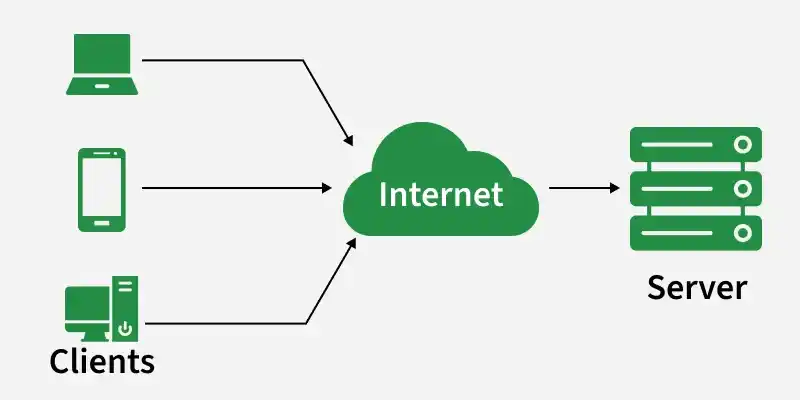
\includegraphics[width=0.75\textwidth]{figures/client-server.png}
  \caption{Client--Server загварын харилцан үйлчлэл}
  \label{fig:client-server}
\end{figure}
Веб системд хэрэглэгчийн хөтөч нь клиентийн үүрэг гүйцэтгэж, сервертэй HTTP хүсэлт болон хариугаар харилцдаг. Хэрэглэгчийн илгээсэн хүсэлтийг сервер боловсруулж, шаардлагатай өгөгдөл эсвэл хуудсыг буцаан илгээдэг. Ийнхүү клиент болон серверийн үүргийг тусгаарласнаар системийг хөгжүүлэх, засварлах болон өргөтгөх боломж сайжирдаг.

\subsection{REST API зарчим}

REST (Representational State Transfer) нь веб системийн програмчлалын интерфейсийн архитектурын хэв загвар бөгөөд Fielding \cite{fielding2000} анх тодорхойлсон. REST зарчимд суурилсан интерфейсийг RESTful API гэж нэрлэх бөгөөд орчин үеийн веб системүүд хоорондын өгөгдөл солилцооны гол арга хэлбэр болж байна.

RESTful API нь нөөц бүрийг URL хаягаар тодорхойлж, тухайн нөөцтэй хийх үйлдлийг HTTP арга (GET, POST, PUT, DELETE)-аар илэрхийлдэг. Жишээлбэл, энэхүү судалгааны ажлын системд амрагч шинэ захиалга үүсгэхдээ \texttt{POST /api/bookings} хүсэлтийг серверт илгээдэг. Сервер уг хүсэлтийг боловсруулж, захиалгын дугаар болон төлвийн мэдээллийг JSON форматаар буцаана. Зураг~\ref{fig:rest-api}-д энэхүү хүсэлт-хариуны урсгалыг харуулав.

\begin{figure}[H]
  \centering
  \begin{tikzpicture}[
    node distance=0.55cm,
    client/.style={rectangle, draw=gray!60, fill=gray!10, rounded corners=4pt,
                   minimum width=5.5cm, minimum height=0.75cm,
                   align=center, font=\small\bfseries},
    payload/.style={rectangle, draw=blue!40, fill=blue!6, rounded corners=3pt,
                    minimum width=5.5cm, align=left,
                    font=\ttfamily\scriptsize, inner sep=7pt},
    server/.style={rectangle, draw=orange!60, fill=orange!12, rounded corners=4pt,
                   minimum width=5.5cm, minimum height=0.75cm,
                   align=center, font=\small\bfseries},
    response/.style={rectangle, draw=teal!50, fill=teal!7, rounded corners=3pt,
                     minimum width=5.5cm, align=left,
                     font=\ttfamily\scriptsize, inner sep=7pt},
    arr/.style={-{Latex[length=2.8mm,width=2mm]}, thick}
  ]
    \node[client]  (cli)  {Хэрэглэгч (хөтөч)};

    \node[payload, below=of cli] (req)
      {POST /api/bookings\\[2pt]
       \{"roomId": 5,\\
       \ "checkIn": "2026-07-01"\}};

    \node[server, below=of req]  (srv)  {Сервер};

    \node[response, below=of srv] (res)
      {HTTP/1.1\ \ 201 Created\\[2pt]
       \{"bookingId": 101,\\
       \ "status": "PENDING"\}};

    \node[client, below=of res] (cli2) {Хэрэглэгч (хариу хүлээн авна)};

    \draw[arr, blue!55]  (cli)  -- node[right, font=\scriptsize\itshape, text=blue!70]{HTTP хүсэлт} (req);
    \draw[arr, blue!55]  (req)  -- (srv);
    \draw[arr, teal!65]  (srv)  -- node[right, font=\scriptsize\itshape, text=teal!70]{HTTP хариу} (res);
    \draw[arr, teal!65]  (res)  -- (cli2);
  \end{tikzpicture}
  \caption{REST API-ийн хүсэлт болон хариуны жишээ}
  \label{fig:rest-api}
\end{figure}

REST API-ийн үндсэн онцлог нь төлөвгүй байдал буюу statelessness юм — сервер клиентийн өмнөх хүсэлтийн мэдээллийг хадгалдаггүй бөгөөд хүсэлт бүр бие даасан, бүрэн мэдээлэл агуулсан байна. Энэхүү зарчим нь клиент болон серверийн хөгжүүлэлтийг бие биенээсээ хамааралгүй явуулах, системийг өргөтгөх боломжийг нэмэгдүүлдэг.

\subsection{Харилцаат өгөгдлийн сангийн загвар}

Харилцаат өгөгдлийн сангийн загвар (relational database model) нь өгөгдлийг хүснэгт хэлбэрээр зохион байгуулж, хүснэгтүүдийн хоорондын харилцааг тодорхойлсон загвар юм \cite{elmasri2015}. Хүснэгт бүр мөр болон баганаас бүрдэнэ.

Загварын гол ойлголтууд:

\begin{itemize}
  \item \textbf{Анхдагч түлхүүр (Primary Key).} Хүснэгтийн мөр бүрийг давтагдашгүй байдлаар таньж тодорхойлдог талбар. Ихэвчлэн автоматаар үүсдэг тоон утга ашигладаг.
  \item \textbf{Гадаад түлхүүр (Foreign Key).} Нэг хүснэгтийн мөрийг өөр хүснэгтийн мөртэй холбох талбар. Хүснэгтүүдийн хоорондын харилцааг тодорхойлно.
  \item \textbf{Нэг-олон харилцаа (One-to-Many).} Нэг хүснэгтийн нэг мөр өөр хүснэгтийн олон мөртэй харилцаатай байх тохиолдол. Жишээ нь нэг амрагч олон захиалга үүсгэж болно.
\end{itemize}

Хүснэгтүүд болон тэдгээрийн хоорондын харилцааг дүрслэхэд Entity-Relationship диаграмм ашигладаг. Зураг~\ref{fig:er-theory}-д хоёр хүснэгтийн хоорондох нэг-олон харилцааны энгийн жишээг үзүүлэв.

\begin{figure}[H]
  \centering
  \begin{tikzpicture}[
    tbl/.style={
      rectangle, draw, rounded corners=4pt,
      minimum width=3.8cm, align=left,
      font=\small, inner sep=8pt
    },
    hdr/.style={
      rectangle, draw, rounded corners=4pt,
      fill=gray!20, minimum width=3.8cm,
      align=center, font=\small\bfseries,
      inner sep=6pt
    },
    arr/.style={-{Latex[length=3mm]}, thick, gray!70!black}
  ]
    % Хэрэглэгч хүснэгт
    \node[hdr] (u_hdr) at (0,0) {Хэрэглэгч};
    \node[tbl, below=-\pgflinewidth of u_hdr, anchor=north] (u_body)
      {\underline{id} (PK)\\нэр\\утас\\үүрэг};

    % Захиалга хүснэгт
    \node[hdr] (b_hdr) at (6,0) {Захиалга};
    \node[tbl, below=-\pgflinewidth of b_hdr, anchor=north] (b_body)
      {\underline{id} (PK)\\хэрэглэгч\_id (FK)\\өрөө\_id\\статус};

    % Холбоос
    \draw[arr] (u_body.east) -- node[above, font=\scriptsize]{1 : N} (b_body.west);
  \end{tikzpicture}
  \caption{Хүснэгтүүдийн хоорондох нэг-олон харилцааны жишээ}
  \label{fig:er-theory}
\end{figure}

Энэхүү загварыг ашигласнаар өгөгдлийн бүрэн бүтэн байдал, давхардлаас сэргийлэх, хурдан хайлт хийх боломж бүрддэг.

\subsection{Нэвтрэлт ба баталгаажуулалтын ойлголт}

Веб системийн аюулгүй байдлын хүрээнд \textit{нэвтрэлт баталгаажуулалт} (authentication) болон \textit{эрх шалгалт} (authorization) гэсэн хоёр ялгаатай ойлголт байдаг. Зураг~\ref{fig:auth-theory}-д эдгээр хоёр ойлголтын ялгааг харуулав.

\begin{figure}[H]
  \centering
  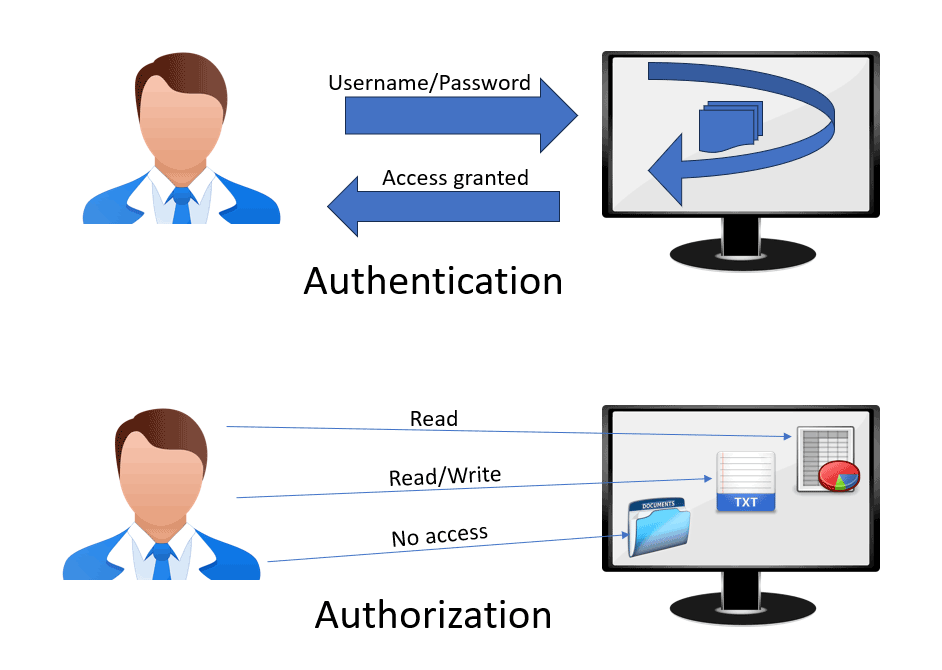
\includegraphics[width=0.72\textwidth]{figures/auth-vs-authz.png}
  \caption{Нэвтрэлт баталгаажуулалт ба эрх шалгалтын ялгаа}
  \label{fig:auth-theory}
\end{figure}

Нэвтрэлт баталгаажуулалт (authentication) нь хэрэглэгч хэн болохыг тогтоох үйл явц бөгөөд эрх шалгалт (authorization) нь тухайн хэрэглэгч системийн ямар нөөцөд хандах боломжтойг тодорхойлдог. Жишээлбэл, зарим хэрэглэгч зөвхөн мэдээлэл харах эрхтэй бол админ хэрэглэгч нэмэх, засах, устгах зэрэг нэмэлт эрхтэй байж болно.

Токенд суурилсан баталгаажуулалтын хүрээнд JSON Web Token (JWT) нь өргөн хэрэглэгддэг стандарт бөгөөд IETF-ийн RFC~7519-ээр тодорхойлогдсон \cite{jones2015jwt}. JWT нь хэрэглэгчийн мэдээллийг агуулсан токен ашиглан серверт сейшн хадгалахгүйгээр хэрэглэгчийг таних боломж олгодог. Энэхүү системд JWT-д суурилсан нэвтрэлт болон эрхийн хяналтыг ашиглаж, хэрэглэгчийг амрагч болон админ гэсэн хоёр үүргээр ялган хэрэгжүүлсэн.

% Бүлэг 3
% ============================================================
% 3-р бүлэг: Судалгааны арга зүй
% ============================================================

\chapter{Судалгааны арга зүй}

% ======= 3.1 =======
\section{Судалгааны арга зүйн ерөнхий тойм}

Тус судалгааны ажил нь практик судалгаа (applied research) хэлбэрээр хэрэгжсэн бөгөөд Өвөрхангай аймгийн Хужирт сумын сувиллуудын одоогийн утсаар захиалга авах, цаасан бүртгэл хөтлөх үйл явцыг цахимжуулах зорилготой веб суурьтай мэдээллийн системийг хөгжүүлэхэд чиглэсэн. Хөгжүүлэлтийн аргачлалд Agile \cite{agilemanifesto2001} философийн зарчмуудыг баримтлан давтамжтай хөгжүүлэлтийн (iterative development) арга барилыг сонгосон. Энэхүү арга нь уламжлалт waterfall загвараас ялгаатай нь хэрэглэгчийн санал хүсэлтэд тулгуурлан системийг алхам алхмаар сайжруулах боломжийг олгодог.

Хөгжүүлэлтийн үйл явц нь долоон үндсэн үе шатаас бүрдсэн. Нэгдүгээр үе шатанд одоогийн сувиллын захиалгын процессын шинжилгээг хийж, утасаар болон биечлэн захиалга авах урсгалыг ажилтнуудтай ярилцлага хийх замаар нарийвчлан судалсан. Хоёрдугаар үе шатанд шаардлагын инженерчлэлийг гүйцэтгэж, функционал болон функционал бус шаардлагуудыг тодорхойлсон. Гуравдугаар үе шатанд системийн архитектурыг загварчилж, T3 Stack (Next.js, TypeScript, Prisma) технологийн стекийг сонгон full-stack веб системийн бүтцийг боловсруулсан. Дөрөвдүгээр үе шатанд өгөгдлийн сангийн схемийг Prisma ORM \cite{prisma2024} ашиглан тодорхойлж, PostgreSQL \cite{postgresql2024} дээр Supabase платформоор дамжуулан байршуулсан. Тавдугаар үе шатанд Next.js API Routes \cite{nextjs2024} болон NextAuth.js \cite{nextauth2024} ашиглан серверийн логик, нэвтрэлтийн системийг хөгжүүлсэн. Зургаадугаар үе шатанд React компонентууд, TailwindCSS ашиглан хэрэглэгчийн интерфейсийг бүтээсэн. Долоодугаар үе шатанд нэгтгэлийн туршилт, ачааллын туршилт, хэрэглэгчийн сэтгэл ханамжийн судалгааг гүйцэтгэсэн.

Давталт бүрийн хугацаа 2 долоо хоног байсан бөгөөд давталт бүрийн эцэст ажиллагаатай хувилбарыг (working increment) гаргаж, удирдагч багш болон сувиллын ажилтнуудаас санал хүсэлт авч дараагийн давталтын ажлыг төлөвлөсөн. Энэхүү давтамжтай арга нь хөгжүүлэлтийн явцад гарсан техникийн болон хэрэглэгчийн туршлагын асуудлуудыг эрт илрүүлж засварлах боломжийг олгосон.

% ======= 3.2 =======
\section{Судалгааны асуултууд}

Тус судалгааны ажлын хүрээнд дараах гурван судалгааны асуултыг дэвшүүлж, туршилтын үр дүнгээр хариулахыг зорьсон.

\textbf{RQ1 (Гүйцэтгэл):} Вэб суурьтай захиалгын систем нь одоогийн цаасан бүртгэл, утасаар захиалга авах процесстой харьцуулахад захиалга боловсруулах хугацааг статистик ач холбогдолтойгоор бууруулж чадах уу?

Энэхүү асуулт нь системийн гол зорилго болох үйл ажиллагааны үр ашгийг хэмжихэд чиглэсэн. Хариултыг тодорхойлохдоо нэг захиалга боловсруулах, мэдээлэл хайх, тайлан гаргах зэрэг үйлдлүүдийн хугацааг хуучин болон шинэ системд хэмжиж харьцуулсан.

\textbf{RQ2 (Алдаа):} Систем нь давхар захиалга (double-booking), огнооны зөрөө зэрэг хүний алдаанаас үүдэлтэй асуудлуудыг бүрэн арилгаж чадах уу?

Цаасан бүртгэлийн хамгийн том сул тал нь ижил өрөөг ижил хугацаанд хоёр өөр хэрэглэгчид захиалахад системийн хяналт байхгүйгээс давхардал үүсэх явдал юм. Энэ асуултад хариулахдаа зэрэг хандалтын (concurrency) туршилтаар системийн pessimistic locking механизмыг шалгасан.

\textbf{RQ3 (Хэрэглэгчийн сэтгэл ханамж):} Системийн ашиглах чадварын (usability) үнэлгээ нь System Usability Scale (SUS) \cite{brooke1996sus} аргачлалын хүлээн зөвшөөрөгдөхүйц босго болох 68 онооноос дээш үнэлгээ авч чадах уу?

SUS нь олон улсад өргөн хэрэглэгддэг хэрэглэгчийн туршлагын (UX) хэмжүүр бөгөөд 10 асуултын 5 оноотой Likert scale-ээр үнэлгээ авч 0--100 хүртэлх оноогоор илэрхийлдэг. Bangor нарын судалгаагаар \cite{bangor2008sus} 68-аас дээш оноо нь ``хүлээн зөвшөөрөгдөхүйц'' (acceptable) гэж тооцогддог.

% ======= 3.3 =======
\section{Системийн үйл ажиллагааны тухай дэлгэрэнгүй}

\subsection{Системд ерөнхий бүтэц}

Энэхүү систем нь T3 Stack дээр суурилсан бүрэн хэмжээний веб систем бөгөөд Next.js, Prisma ORM, NextAuth.js технологиудыг ашигласан. Хэрэглэгчийн хүсэлт нь Next.js App Router-аар дамжин Prisma ORM-р PostgreSQL өгөгдлийн санд хандах бүтэцтэй ба T3 технологийн стек нь TypeScript хэлийг ашиглан frontend, backend хооронд кодын давхардлыг багасгаж, системийн найдвартай байдлыг хангадаг.

\begin{figure}[htbp]
\centering
\begin{tikzpicture}[
    node distance=0.9cm,
    font=\normalsize,
    layer/.style={
        rectangle,
        rounded corners=6pt,
        draw,
        line width=1.2pt,
        minimum width=11cm,
        minimum height=1.6cm,
        align=center,
        inner sep=6pt
    },
    client/.style   ={layer, draw=violet!60,      fill=violet!12},
    frontend/.style ={layer, draw=orange!70,      fill=orange!15},
    backend/.style  ={layer, draw=red!55,         fill=red!12},
    database/.style ={layer, draw=green!55!black, fill=green!15},
    arr/.style={-{Latex[length=3mm, width=2mm]}, line width=1.2pt}
]
\node[client] (client)
    {\textbf{Хэрэглэгчийн давхарга (client)} \\[2pt]
     Зочин \ $\cdot$ \ Админ \ $\cdot$ \ Ресепшн};

\node[frontend, below=of client] (frontend)
    {\textbf{Харагдах хэсэг (frontend)} \\[2pt]
     Next.js 14 \ $\cdot$ \ React \ $\cdot$ \ TailwindCSS};

\node[backend, below=of frontend] (backend)
    {\textbf{Серверийн хэсэг (backend)} \\[2pt]
     Next.js API Routes \ $\cdot$ \ NextAuth.js \ $\cdot$ \ Prisma ORM};

\node[database, below=of backend] (database)
    {\textbf{Өгөгдлийн давхарга (database)} \\[2pt]
     PostgreSQL \ $\cdot$ \ Supabase};

\draw[arr, violet!60] (client)   -- (frontend);
\draw[arr, orange!70] (frontend) -- (backend);
\draw[arr, red!55]    (backend)  -- (database);
\end{tikzpicture}
\caption{Системийн дөрвөн давхаргат бүтэц}
\label{fig:architecture}
\end{figure}

\subsection{Системийн үндсэн урсгал}

Системийн үндсэн үйл ажиллагааны урсгал нь дараах дарааллаар явагдана: зочин буюу үйлчлүүлэгч вэб хуудсанд орж сувиллын мэдээлэл болон өрөөний жагсаалттай танилцана, захиалга хийхийн тулд ирэх унаа, огноо болон хүний тоо сонгон боломжтой өрөөг хайлт хийж, захиалга үүсгэнэ. Үүсгэсэн захиалга дээр амжилттай төлбөр төлөгдсөн тохиолдолд систем хэрэглэгчид мэдэгдэл илгээж захиалга бүртгэгдсэн гэдгийг баталгаажуулна. Энэхүү урсгал нь одоогийн утсаар захиалга авах, цаасан бүртгэл хөтлөх уламжлалт аргыг цахим орчинд шилжүүлж байгаа юм.

\begin{figure}[H]
  \centering
  \figplaceholder[0.55]{system_flow}
  \caption{Системийн үндсэн урсгалын диаграмм}
  \label{fig:system-flow}
\end{figure}

% ======= 3.4 =======
\section{Системийн хэрэглэгчид}

Системд дөрвөн үүргийн (role) хэрэглэгч байх бөгөөд үүрэг бүр нь тодорхой эрх, боломжоор хязгаарлагдана. Зочин (Guest) хэрэглэгч бүртгэлгүй байдлаар сувиллын ерөнхий мэдээлэл, өрөөний жагсаалт, үнийн мэдээллийг харж болох боловч захиалга хийхийн тулд бүртгүүлэх шаардлагатай болно. Энэхүү нээлттэй танилцах боломж нь боломжит үйлчлүүлэгчдийг татах маркетингийн чиг үүрэгтэй.

Үйлчлүүлэгч гэдэг нь бүртгүүлсний дараа идэвхждэг үүрэг бөгөөд захиалга үүсгэх, өөрийн захиалгын түүх харах, профайлын мэдээлэл засах, баталгаажсан захиалгаас хугацаанаас өмнө цуцлах боломжтой. Ажилтан нь өөрийн сувиллын орж ирсэн захиалгуудыг хянаж баталгаажуулах эсвэл цуцлах, ирэх үйлчлүүлэгчдийн нэрсийн жагсаалт гаргах үүрэгтэй. Захиалгын цаг хугацаа, нийт орны хүчин чадлыг ажилтан хянаснаар давхардсан захиалга болон алдааг урьдчилан сэргийлнэ. Админ нь системийн хамгийн өндөр эрхтэй үүрэг бөгөөд бүх сувиллын захиалга, хэрэглэгч, өрөөний мэдээлэл удирдах, тайлан статистик харах, ажилтан бүртгэх боломжтой.

\vspace{0.5cm}

\begin{table}[H]
  \centering
  \caption{Хэрэглэгчийн эрхийн хүснэгт}
  \label{tab:role-matrix}
  \begin{tabular}{|l|c|c|c|c|}
    \hline
    \textbf{Үйлдэл} & \textbf{Зочин} & \textbf{Үйлчлүүлэгч} & \textbf{Ажилтан} & \textbf{Админ} \\
    \hline
    Сувиллын мэдээлэл харах  & + & + & + & + \\
    \hline
    Захиалга хийх            & -- & + & -- & + \\
    \hline
    Өөрийн захиалга цуцлах   & -- & + & -- & + \\
    \hline
    Захиалга баталгаажуулах   & -- & -- & + & + \\
    \hline
    Ажилтан бүртгэх          & -- & -- & -- & + \\
    \hline
    Тайлан харах             & -- & -- & -- & + \\
    \hline
  \end{tabular}
\end{table}

% ======= 3.5 =======
\section{Системийн шаардлага}

Судалгааны явцад системд шаардлагатай үндсэн функцуудыг сувиллын ажилтантай хийсэн асуулга, ярилцлагын аргаар тодорхойлсон.
Мөн системийн найдвартай байдал, аюулгүй байдлын шаардлагуудыг тусгайлан авч үзсэн. Эдгээр шаардлагуудыг тодорхойлохдоо Эрүүл мэндийн яамны нийтийн эрүүл мэнд, нөхөн сэргээх үйлчилгээний статистик мэдээллийг \cite{mohstats2023} суурь мэдээлэл болгон ашигласан.
Доорх зурагт Хужирт сумын нэгэн сувилалд 2016–2023 оны хооронд үйлчлүүлсэн үйлчлүүлэгчдийн тооны өөрчлөлтийг харуулав.
\begin{figure}[H]
  \centering
  \begin{tikzpicture}
    \begin{axis}[
      ybar,
      bar width=0.58cm,
      width=0.85\textwidth,
      height=6.5cm,
      xtick={1,2,3,4,5,6,7,8},
      xticklabels={2016,2017,2018,2019,2020,2021,2022,{2023/11}},
      nodes near coords,
      nodes near coords align={vertical},
      every node near coord/.style={font=\scriptsize},
      ymin=0,
      ymax=6500,
      ylabel={Үйлчлүүлэгчийн тоо (хүн)},
      xlabel={Он},
      enlarge x limits=0.08,
      tick label style={font=\small},
      label style={font=\small},
    ]
      \addplot[fill=blue!45, draw=blue!70] coordinates {
        (1,1450)(2,2937)(3,3346)(4,4069)
        (5,3863)(6,2521)(7,5146)(8,4247)
      };
    \end{axis}
  \end{tikzpicture}
  \caption{Хужирт сумын нэг сувиллын үйлчлүүлэгчийн тооны өөрчлөлт (2016--2023)\\[2pt]}
  \label{fig:customers-stats}
\end{figure}
\vspace{0.5cm}

\begin{table}[H]
  \centering
  \caption{Системийн шаардлагын жагсаалт}
  \label{tab:functional-req}
  \begin{tabular}{|l|l|p{6cm}|l|}
    \hline
    \textbf{FR-ID} & \textbf{Шаардлагын нэр} & \textbf{Тодорхойлолт} & \textbf{Хамаарах үүрэг} \\
    \hline
    FR-01 & Нэвтрэх               & Имэйл/нууц үгээр нэвтрэх                          & Бүгд \\
    \hline
    FR-02 & Бүртгүүлэх            & Шинэ хэрэглэгч үүсгэх, имэйл баталгаажуулалт                  & Зочин \\
    \hline
    FR-03 & Захиалга үүсгэх       & Өрөө, огноо, хүний тоо сонгон захиалга өгөх                   & Үйлчлүүлэгч \\
    \hline
    FR-04 & Захиалга баталгаажуулах & Ажилтан захиалгыг хянаж батлах                               & Ажилтан \\
    \hline
    FR-05 & Захиалга цуцлах       & Үйлчлүүлэгч эсвэл ажилтан захиалга цуцлах                    & Үйлчлүүлэгч, Ажилтан \\
    \hline
    FR-06 & Өрөөний хүртээмж      & Сонгосон огноонд хоосон өрөө шүүх                             & Зочин, Үйлчлүүлэгч \\
    \hline
    FR-07 & Тайлан гаргах         & Сарын захиалга, орлого, дүүргэлтийн хувь                      & Админ \\
    \hline
    FR-08 & Хэрэглэгч удирдах     & Хэрэглэгч, ажилтан бүртгэх, засах                             & Админ \\
    \hline
    FR-09 & Мэдэгдэл илгээх       & Захиалга баталгаажсан, ирэх өдрийг сануулах                   & Систем \\
    \hline
    FR-10 & Профайл засах         & Нэр, утас, нууц үг шинэчлэх                                   & Үйлчлүүлэгч \\
    \hline
  \end{tabular}
\end{table}

% ======= 3.6 =======

Статистик мэдээллээс харахад 2022 онд үйлчлүүлэгчдийн тоо 5,146-д хүрч, судлагдсан хугацаанд хамгийн өндөр үзүүлэлтэд хүрсэн байна. Энэхүү өсөлтийн хандлага нь системд ирэх ачаалал нэмэгдэхийг илтгэж байгаа тул уг өгөгдөлд тулгуурлан функционал бус шаардлагуудыг тодорхойлсон.
Нэгдүгээрт, жилийн дундаж болон оргил ачааллын үед нэгэн зэрэг нэвтрэх хэрэглэгчдийн тоо мэдэгдэхүйц өсөх хандлагатай тул \textbf{NFR-01 гүйцэтгэлийн шаардлага}-ын хүрээнд 100-аас дээш хэрэглэгчийг нэгэн зэрэг 200 ms-ээс бага хариу хугацаатайгаар дэмжих шаардлагыг тогтоосон.
Хоёрдугаарт, олон хэрэглэгч нэгэн зэрэг ижил өрөөг захиалах нөхцөл үүсэх магадлалтай учир \textbf{NFR-03 захиалга түгжих} механизмыг хэрэгжүүлэх шаардлагатай гэж үзсэн.
Гуравдугаарт, хэрэглэгчдийн тодорхой хувь нь гар утас болон таблет төхөөрөмжөөс системд хандах хэрэгцээтэй тул \textbf{NFR-04 responsive дизайн}-ыг зайлшгүй хангахаар тусгасан.
\vspace{0.5cm}
\begin{table}[H]
  \centering
  \caption{Функционал бус шаардлагууд}
  \label{tab:nonfunctional-req}
  \begin{tabular}{|l|l|p{5.5cm}|p{3.5cm}|}
    \hline
    \textbf{NFR-ID} & \textbf{Ангилал} & \textbf{Шаардлага} & \textbf{Хэмжих үзүүлэлт} \\
    \hline
    NFR-01 & Гүйцэтгэл      
    & API хариу хугацаа дунджаар 200 ms-ээс бага, 100+ хэрэглэгчийг нэгэн зэрэг дэмжих    
    & Ачааллын тест (Load test) \\
    \hline
    NFR-02 & Аюулгүй байдал 
    & HTTPS протокол, JWT токен, bcrypt алгоритмаар нууц үг хэшлэх, SQL injection хамгаалалт                  
    & Аюулгүй байдлын тест \\
    \hline
    NFR-03 & Өгөгдлийн бүрэн бүтэн байдал 
    & Захиалгыг баталгаажуулах хүртэл 10 минутын хугацаанд түгжих механизм хэрэгжүүлэх                            
    & Зэрэг хандалтын тест \\
    \hline
    NFR-04 & Хүртээмж       
    & Responsive дизайн (гар утас, таблет, компьютер дээр зохицох)          
    & Дэлгэцийн тест \\
    \hline
    NFR-05 & Засвар үйлчилгээ 
    & Лог бүртгэл, кодын баримтжуулалт, хялбар deploy хийх боломж                              
    & Кодын хяналт \\
    \hline
  \end{tabular}
\end{table}

% ======= 3.7 =======
\section{Юзкейс диаграммууд}

\subsection{Үйлчлүүлэгчийн юзкейс диаграмм}

Үйлчлүүлэгч бүртгүүлсний дараа захиалга үүсгэх, өөрийн захиалгын түүх болон статусыг харах, профайлын мэдээлэл засах, хугацааны нөхцөлийг хангасан захиалгаа цуцлах боломжтой.

\begin{figure}[H]
\centering
\begin{tikzpicture}[
    font=\normalsize,
    usecase/.style={
        ellipse,
        draw=blue!55!black,
        line width=0.9pt,
        fill=blue!18,
        minimum width=4.2cm,
        minimum height=1.6cm,
        align=center,
        inner sep=3pt
    },
    arr/.style={-{Latex[length=3mm, width=2mm]}, line width=0.9pt},
    ext/.style={-{Latex[length=2.5mm, width=1.8mm]}, line width=0.7pt, dashed}
]

\draw[line width=0.9pt] (0, 0) circle (0.35cm);
\draw[line width=0.9pt] (0, -0.35) -- (0, -1.5);
\draw[line width=0.9pt] (-0.7, -0.85) -- (0.7, -0.85);
\draw[line width=0.9pt] (0, -1.5) -- (-0.5, -2.3);
\draw[line width=0.9pt] (0, -1.5) -- (0.5, -2.3);
\node[below=0.1cm] at (0, -2.4) {\textbf{Үйлчлүүлэгч}};

\node[usecase] (register) at (7.5,  4.8)   {Бүртгэл үүсгэх / \\ Нэвтрэх};
\node[usecase] (viewroom) at (7.5,  2.7)   {Өрөө харах / \\ Хайх};
\node[usecase] (book)     at (7.5,  0.7)   {Захиалга үүсгэх};
\node[usecase] (mybook)   at (7.5, -1.3)   {Захиалгаа харах / \\ Засах};
\node[usecase] (cancel)   at (7.5, -3.3)   {Захиалгаа цуцлах};
\node[usecase] (payment)  at (7.5, -5.3)   {Урьдчилгаа төлбөр \\ төлөх};

\draw[arr] (0.7, -0.85) -- (register.west);
\draw[arr] (0.7, -0.85) -- (viewroom.west);
\draw[arr] (0.7, -0.85) -- (book.west);
\draw[arr] (0.7, -0.85) -- (mybook.west);
\draw[arr] (0.7, -0.85) -- (cancel.west);
\draw[arr] (0.7, -0.85) -- (payment.west);

\draw[ext] (viewroom.south) -- (book.north);
\draw[ext] (payment.north east) to[bend right=30] (book.south east);

\end{tikzpicture}
\caption{Үйлчлүүлэгчийн юзкейс диаграмм}
\label{fig:usecase-customer}
\end{figure}

\subsection{Ажилтан болон Админы юзкейс диаграмм}

Ажилтан өөрийн сувиллд ирсэн захиалгуудыг хянаж баталгаажуулах, шаардлагатай тохиолдолд цуцлах, ирэх хугацааны үйлчлүүлэгчдийн жагсаалт гаргах боломжтой бөгөөд өрөөний хүртээмжийн хяналтыг удирддаг. Админ системийн хамгийн өндөр эрхийн хэрэглэгч бөгөөд бүх сувиллын захиалга, өрөөний мэдээлэл, хэрэглэгчийн бүртгэлийг удирдах, ажилтан нэмэх, тайлан статистик харах зэрэг бүх үйлдлийг гүйцэтгэх боломжтой.

\begin{figure}[H]
\centering
\begin{tikzpicture}[
    font=\normalsize,
    shared/.style={
        ellipse,
        draw=green!50!black,
        line width=0.9pt,
        fill=green!20,
        minimum width=4.2cm,
        minimum height=1.5cm,
        align=center,
        inner sep=3pt
    },
    adminuc/.style={
        ellipse,
        draw=orange!70!black,
        line width=0.9pt,
        fill=orange!25,
        minimum width=4.2cm,
        minimum height=1.5cm,
        align=center,
        inner sep=3pt
    },
    arr/.style={-{Latex[length=3mm, width=2mm]}, line width=0.9pt}
]

\draw[line width=0.9pt] (0,  4.5) circle (0.35cm);
\draw[line width=0.9pt] (0,  4.15) -- (0,  3.0);
\draw[line width=0.9pt] (-0.7, 3.65) -- (0.7, 3.65);
\draw[line width=0.9pt] (0,  3.0) -- (-0.5, 2.2);
\draw[line width=0.9pt] (0,  3.0) -- ( 0.5, 2.2);
\node[below=0.1cm, align=center] at (0, 2.1) {Хүлээн авах \\ ажилтан};

\draw[line width=0.9pt] (0, -1.5) circle (0.35cm);
\draw[line width=0.9pt] (0, -1.85) -- (0, -3.0);
\draw[line width=0.9pt] (-0.7, -2.35) -- (0.7, -2.35);
\draw[line width=0.9pt] (0, -3.0) -- (-0.5, -3.8);
\draw[line width=0.9pt] (0, -3.0) -- ( 0.5, -3.8);
\node[below=0.1cm] at (0, -3.9) {Админ};

\node[shared]  (confirm)  at (8,  5.2)   {Захиалга баталгаажуулах};
\node[shared]  (viewlist) at (8,  3.0)   {Захиалгын жагсаалт \\ харах};
\node[shared]  (status)   at (8,  0.8)   {Захиалгын төлөв \\ өөрчлөх};

\node[adminuc] (rooms)    at (8, -1.4)   {Өрөө / Үйлчилгээ \\ нэмэх, засах};
\node[adminuc] (staff)    at (8, -3.3)   {Ажилтан удирдах};
\node[adminuc] (report)   at (8, -5.2)   {Тайлан, статистик \\ гаргах};

\draw[arr] (0.7,  3.65) -- (confirm.west);
\draw[arr] (0.7,  3.65) -- (viewlist.west);
\draw[arr] (0.7,  3.65) -- (status.west);

\draw[arr] (0.7, -2.35) -- (status.west);
\draw[arr] (0.7, -2.35) -- (viewlist.west);
\draw[arr] (0.7, -2.35) -- (rooms.west);
\draw[arr] (0.7, -2.35) -- (staff.west);
\draw[arr] (0.7, -2.35) -- (report.west);

\end{tikzpicture}
\caption{Ажилтан болон Админы юзкейс диаграмм}
\label{fig:usecase-staff-admin}
\end{figure}

% ======= 3.8 =======
\section{Дарааллын диаграммууд}

\subsection{Бүртгэл ба нэвтрэлтийн дараалал}

Хэрэглэгч имэйл болон нууц үгээ оруулахад NextAuth.js хүсэлтийг хүлээн авч Prisma ORM-р дамжуулан PostgreSQL өгөгдлийн санд хадгалагдсан хэрэглэгчийн мэдээлэлтэй шалгана, амжилттай баталгаажсан тохиолдолд JWT session токен үүсгэн хэрэглэгчийн хөтөч дээр хадгалагдана.

\begin{figure}[H]
\centering
\resizebox{0.95\textwidth}{!}{
\begin{tikzpicture}[
    font=\small,
    actor/.style={
        rectangle,
        draw=blue!40!black,
        fill=blue!8,
        rounded corners=4pt,
        minimum width=2.6cm,
        minimum height=0.7cm,
        align=center
    },
    line/.style={dashed, gray!80, line width=0.6pt},
    msg/.style={-Latex, line width=0.8pt},
    ret/.style={-Latex, dashed, line width=0.8pt}
]

\def\xa{0}
\def\xb{4.3}
\def\xc{8.6}
\def\xd{12.9}

% Actors
\node[actor] (u)  at (\xa, 0) {Хэрэглэгч \\ (веб)};
\node[actor] (na) at (\xb, 0) {NextAuth.js};
\node[actor] (pr) at (\xc, 0) {Prisma ORM};
\node[actor] (db) at (\xd, 0) {PostgreSQL};

% Lifelines
\draw[line] (\xa, -0.6) -- (\xa, -13.2);
\draw[line] (\xb, -0.6) -- (\xb, -13.2);
\draw[line] (\xc, -0.6) -- (\xc, -13.2);
\draw[line] (\xd, -0.6) -- (\xd, -13.2);

% [БҮРТГЭЛ]
\node[anchor=west, font=\bfseries\small, text=gray!80!black] at (-0.5, -1.0) {Бүртгэл};

\draw[msg] (\xa, -1.8) -- node[above, font=\scriptsize] {1. Бүртгэлийн мэдээлэл (нэр, имэйл, нууц үг)} (\xb, -1.8);
\draw[msg] (\xb, -2.6) -- node[above, font=\scriptsize] {2. Шинэ хэрэглэгч үүсгэх хүсэлт} (\xc, -2.6);
\draw[msg] (\xc, -3.4) -- node[above, font=\scriptsize] {3. INSERT INTO users} (\xd, -3.4);

\draw[ret] (\xd, -4.2) -- node[above, font=\scriptsize] {4. Хэрэглэгч амжилттай үүссэн} (\xc, -4.2);
\draw[ret] (\xc, -5.0) -- node[above, font=\scriptsize] {5. User объект буцаах} (\xb, -5.0);
\draw[ret] (\xb, -5.8) -- node[above, font=\scriptsize] {6. Бүртгэл амжилттай (нэвтрэх хуудас руу)} (\xa, -5.8);

% Separator
\draw[loosely dashed, gray!50] (-0.8, -6.6) -- (\xd+0.8, -6.6);

% [НЭВТРЭЛТ]
\node[anchor=west, font=\bfseries\small, text=gray!80!black] at (-0.5, -7.2) {Нэвтрэлт};

\draw[msg] (\xa, -8.0) -- node[above, font=\scriptsize] {7. Имэйл, нууц үг оруулах} (\xb, -8.0);
\draw[msg] (\xb, -8.8) -- node[above, font=\scriptsize] {8. Имэйлээр хэрэглэгч хайх} (\xc, -8.8);
\draw[msg] (\xc, -9.6) -- node[above, font=\scriptsize] {9. SELECT * FROM users WHERE email=?} (\xd, -9.6);

\draw[ret] (\xd, -10.4) -- node[above, font=\scriptsize] {10. Хэрэглэгчийн мэдээлэл} (\xc, -10.4);
\draw[ret] (\xc, -11.2) -- node[above, font=\scriptsize] {11. User + hashed нууц үг} (\xb, -11.2);

\node[draw=gray!50, fill=yellow!15, text=black, align=center, font=\scriptsize, rounded corners=3pt, inner sep=4pt] at (\xb, -12.0) {bcrypt.compare() \\ нууц үг шалгах};

\draw[ret] (\xb, -12.8) -- node[above, font=\scriptsize] {12. JWT session токен (cookie-д хадгалах)} (\xa, -12.8);

\end{tikzpicture}
}
\caption{Бүртгэл ба нэвтрэлтийн дараалал диаграмм}
\label{fig:seq-auth}
\end{figure}

\subsection{Захиалга үүсгэх дараалал}

Үйлчлүүлэгч огноо, өрөө, хүний тоо сонгон захиалга илгээхэд tRPC mutation дуудагдаж серверийн хэсэгт хүсэлт очно, Prisma ашиглан өгөгдлийн санд шинэ захиалгын бичлэг үүсч, захиалгын статус ``хүлээгдэж байна'' (pending) болж тохируулагдана.

\begin{figure}[H]
\centering
\resizebox{0.95\textwidth}{!}{
\begin{tikzpicture}[
    font=\small,
    actor/.style={
        rectangle,
        draw=blue!40!black,
        fill=blue!8,
        rounded corners=4pt,
        minimum width=2.6cm,
        minimum height=0.7cm,
        align=center
    },
    line/.style={dashed, gray!80, line width=0.6pt},
    msg/.style={-Latex, line width=0.8pt},
    ret/.style={-Latex, dashed, line width=0.8pt}
]

\def\xa{0}
\def\xb{4.8}
\def\xc{9.6}
\def\xd{14.4}

% Actors
\node[actor] (u)  at (\xa, 0) {Үйлчлүүлэгч \\ (веб)};
\node[actor] (na) at (\xb, 0) {tRPC \\ (API Router)};
\node[actor] (pr) at (\xc, 0) {Prisma ORM};
\node[actor] (db) at (\xd, 0) {PostgreSQL};

% Lifelines
\draw[line] (\xa, -0.6) -- (\xa, -8.5);
\draw[line] (\xb, -0.6) -- (\xb, -8.5);
\draw[line] (\xc, -0.6) -- (\xc, -8.5);
\draw[line] (\xd, -0.6) -- (\xd, -8.5);

\draw[msg] (\xa, -1.3) -- node[above, font=\scriptsize] {1. Огноо, өрөө, хүний тоо сонгон захиалга илгээх} (\xb, -1.3);

\draw[msg] (\xb, -2.9) -- node[above, font=\scriptsize] {2. booking.create mutation дуудах} (\xc, -2.9);
\draw[msg] (\xc, -3.7) -- node[above, font=\scriptsize] {3. Өрөөний хүртээмж шалгах (SELECT)} (\xd, -3.7);

\draw[ret] (\xd, -4.5) -- node[above, font=\scriptsize] {4. Өрөө хоосон байна} (\xc, -4.5);

\draw[msg] (\xc, -5.3) -- node[above, font=\scriptsize] {5. INSERT INTO bookings (status=pending)} (\xd, -5.3);

\draw[ret] (\xd, -6.1) -- node[above, font=\scriptsize] {6. Захиалга амжилттай үүссэн} (\xc, -6.1);
\draw[ret] (\xc, -6.9) -- node[above, font=\scriptsize] {7. Booking объект буцаах} (\xb, -6.9);
\draw[ret] (\xb, -7.7) -- node[above, font=\scriptsize] {8. Захиалга үүссэн (status: pending)} (\xa, -7.7);

\end{tikzpicture}
}
\caption{Захиалга үүсгэх дараалал диаграмм}
\label{fig:seq-booking}
\end{figure}

\subsection{Захиалга баталгаажуулах дараалал}

Ажилтан хүлээгдэж буй захиалгуудын жагсаалтаас захиалга сонгон баталгаажуулахад tRPC mutation дуудагдаж өгөгдлийн санд захиалгын статус ``баталгаажсан'' (confirmed) болж шинэчлэгдэх бөгөөд систем автоматаар үйлчлүүлэгчид мэдэгдэл илгээнэ.

\begin{figure}[H]
\centering
\resizebox{0.95\textwidth}{!}{
\begin{tikzpicture}[
    font=\small,
    actor/.style={
        rectangle,
        draw=blue!40!black,
        fill=blue!8,
        rounded corners=4pt,
        minimum width=2.6cm,
        minimum height=0.7cm,
        align=center
    },
    line/.style={dashed, gray!80, line width=0.6pt},
    msg/.style={-Latex, line width=0.8pt},
    ret/.style={-Latex, dashed, line width=0.8pt}
]

\def\xa{0}
\def\xb{4.8}
\def\xc{9.6}
\def\xd{14.4}

% Actors
\node[actor] (st)  at (\xa, 0) {Ажилтан \\ (Дэлгэц)};
\node[actor] (na) at (\xb, 0) {tRPC \\ (API Router)};
\node[actor] (pr) at (\xc, 0) {Prisma ORM};
\node[actor] (db) at (\xd, 0) {PostgreSQL};

% Lifelines
\draw[line] (\xa, -0.6) -- (\xa, -8.3);
\draw[line] (\xb, -0.6) -- (\xb, -8.3);
\draw[line] (\xc, -0.6) -- (\xc, -8.3);
\draw[line] (\xd, -0.6) -- (\xd, -8.3);

\draw[msg] (\xa, -1.3) -- node[above, font=\scriptsize] {1. Захиалга баталгаажуулах хүсэлт илгээх} (\xb, -1.3);
\draw[msg] (\xb, -2.3) -- node[above, font=\scriptsize] {2. update.booking(status='confirmed')} (\xc, -2.3);
\draw[msg] (\xc, -3.3) -- node[above, font=\scriptsize] {3. UPDATE bookings SET status='confirmed'} (\xd, -3.3);

\draw[ret] (\xd, -4.3) -- node[above, font=\scriptsize] {4. Бичлэг амжилттай шинэчлэгдсэн} (\xc, -4.3);
\draw[ret] (\xc, -5.3) -- node[above, font=\scriptsize] {5. Захиалгын объект буцаах} (\xb, -5.3);

\node[draw=gray!50, fill=yellow!15, text=black, align=center, font=\scriptsize, rounded corners=3pt, inner sep=4pt] at (\xb, -6.3) {Үйлчлүүлэгч рүү баталгаажсан \\ тухай автомат имэйл илгээх};

\draw[ret] (\xb, -7.3) -- node[above, font=\scriptsize] {6. Дэлгэцэд "Амжилттай" төлөв харуулах} (\xa, -7.3);

\end{tikzpicture}
}
\caption{Захиалга баталгаажуулах дараалал диаграмм}
\label{fig:seq-confirm}
\end{figure}

% ======= 3.9 =======
\section{Өгөгдлийн сангийн ерөнхий загвар}

\subsection{Үндсэн хүснэгтүүд ба харилцаа холбоо}

Өгөгдлийн сангийн бүтэц нь Prisma schema дээр суурилсан таван үндсэн хүснэгтээс бүрдэх бөгөөд тэдгээрийн хоорондын харилцаа нь гадаад түлхүүр (foreign key) ашиглан нэг-олон (one-to-many) хамаарлаар холбогдоно. Хүснэгтүүд нь хэрэглэгч, сувилл, өрөө, захиалга, эмчилгээний бүртгэлийн мэдээллийг тусад нь хадгалж системийн мэдээллийн бүрэн бүтэн байдлыг хангана.

\begin{figure}[H]
\centering
\resizebox{\textwidth}{!}{
\begin{tikzpicture}[
    font=\small,
    % ---- Entity (хүснэгт) хэв маяг ----
    entity/.style={
        rectangle split,
        rectangle split parts=2,
        rectangle split part fill={violet!25, white},
        draw=violet!40,
        line width=0.8pt,
        rounded corners=3pt,
        align=left,
        text width=4.8cm,
        inner sep=6pt
    },
    % ---- Харилцааны шугам ----
    rel/.style={line width=0.7pt, black!70},
    % ---- Multiplicity label ----
    mult/.style={
        font=\small,
        inner sep=3pt,
        fill=white,
        draw=none
    }
]

% ---- Талбар харуулах макронууд ----
\newcommand{\pk}[2]{\underline{#1} : \textit{#2} \ \textsc{\footnotesize(PK)} \\}
\newcommand{\fk}[2]{#1 : \textit{#2} \ \textsc{\footnotesize(FK)} \\}
\newcommand{\attr}[2]{#1 : \textit{#2} \\}

% ---------- ROW 1: users, sanatoriums, rooms ----------
\node[entity] (User) at (0, 10) {
    \textbf{users} \nodepart{second}
    \pk{id}{String}
    \attr{name}{String}
    \attr{email}{String (unique)}
    \attr{password}{String}
    \attr{role}{Role}
    \attr{phone}{String?}
    \attr{createdAt}{DateTime}
};

\node[entity] (Sana) at (6.5, 10) {
    \textbf{sanatoriums} \nodepart{second}
    \pk{id}{String}
    \attr{name}{String}
    \attr{location}{String}
    \attr{description}{String?}
    \attr{phone}{String?}
    \attr{createdAt}{DateTime}
};

\node[entity] (Room) at (13, 10) {
    \textbf{rooms} \nodepart{second}
    \pk{id}{String}
    \fk{sanatoriumId}{String}
    \attr{name}{String}
    \attr{type}{RoomType}
    \attr{capacity}{Int}
    \attr{pricePerNight}{Float}
    \attr{imageUrl}{String?}
};

% ---------- ROW 2: bookings, booking_rooms ----------
\node[entity] (Booking) at (0, 2) {
    \textbf{bookings} \nodepart{second}
    \pk{id}{String}
    \fk{userId}{String}
    \attr{checkIn}{DateTime}
    \attr{checkOut}{DateTime}
    \attr{guests}{Int}
    \attr{totalPrice}{Float}
    \attr{status}{Status}
    \attr{createdAt}{DateTime}
};

\node[entity] (BR) at (13, 2) {
    \textbf{booking\_rooms} \nodepart{second}
    \pk{id}{String}
    \fk{bookingId}{String}
    \fk{roomId}{String}
    \attr{pricePerNight}{Float}
    \attr{nights}{Int}
};

% ---------- ROW 3: booking_treatments, payments ----------
\node[entity] (BT) at (0, -5) {
    \textbf{booking\_treatments} \nodepart{second}
    \pk{id}{String}
    \fk{bookingId}{String}
    \attr{name}{String}
    \attr{quantity}{Int}
    \attr{unitPrice}{Float}
    \attr{totalPrice}{Float}
};

\node[entity] (Pay) at (6.5, -5) {
    \textbf{payments} \nodepart{second}
    \pk{id}{String}
    \fk{bookingId}{String}
    \attr{amount}{Float}
    \attr{method}{PaymentMethod}
    \attr{status}{PaymentStatus}
    \attr{paidAt}{DateTime?}
    \attr{createdAt}{DateTime}
};

% ============================================================
%  ХАРИЛЦААНУУД
% ============================================================

% users ── bookings
\draw[rel] (User.south) -- (Booking.north)
    node[mult, midway]{1 : N};

% sanatoriums ── rooms
\draw[rel] (Sana.east) -- (Room.west)
    node[mult, midway]{1 : N};

% bookings ── booking_rooms
\draw[rel] (Booking.east) -- (BR.west)
    node[mult, midway]{1 : N};

% rooms ── booking_rooms
\draw[rel] (Room.south) -- (BR.north)
    node[mult, midway]{1 : N};

% bookings ── booking_treatments
\draw[rel] (Booking.south) -- (BT.north)
    node[mult, midway]{1 : N};

% bookings ── payments
\draw[rel] ($(Booking.south) + (1.5,0)$) -- ++(0,-2) -| (Pay.north)
    node[mult, pos=0.5]{1 : N};

% N:N тэмдэглэл
\node[font=\footnotesize\itshape, text=violet!70!black]
    at (9.7, 5.8) {bookings $\longleftrightarrow$ rooms \ (N : N)};

\end{tikzpicture}
}

\caption{Өгөгдлийн сангийн ER диаграмм}
\label{fig:er-diagram}
\end{figure}

\subsection{Хүснэгтүүдийн тайлбар}

\begin{table}[H]
  \centering
  \caption{Өгөгдлийн сангийн үндсэн хүснэгтүүд}
  \label{tab:db-tables}
  \begin{tabular}{lp{4cm}ll}
    \toprule
    \textbf{Хүснэгтийн нэр} & \textbf{Тодорхойлолт} & \textbf{Гол түлхүүр} & \textbf{Гадаад түлхүүр} \\
    \midrule
    users               & Системийн бүх хэрэглэгч, үүрэг (role) талбарын утгаар ялгана   & id & — \\
    sanatoriums         & Бүртгэлтэй сувиллуудын нэр, байршил, холбоо барих мэдээлэл     & id & — \\
    rooms               & Сувилл бүрийн өрөөний мэдээлэл, үнэ, хүчин чадал               & id & sanatorium\_id \\
    bookings            & Захиалгын бүртгэл, статус, огноо, нийт үнийн дүн               & id & user\_id, room\_id \\
    booking\_treatments & Захиалгад хамаарах эмчилгээний нэр, тоо, үнийн дэлгэрэнгүй   & id & booking\_id \\
    \bottomrule
  \end{tabular}
\end{table}

% Бүлэг 4
% ============================================================
% 4-р бүлэг: Судалгааны үр дүн, дүгнэлт
% ============================================================

\chapter{Судалгааны үр дүн, дүгнэлт}

\section{Туршилт, үнэлгээ}



\section{Үр дүнгийн шинжилгээ}



\section{Дүгнэлт, цаашдын чиглэл}




% Ном зүй
% --- НОМ ЗҮЙ ---
\newpage
\phantomsection
\addcontentsline{toc}{chapter}{Ном зүй}
\printbibliography[title={Ном зүй}]


% Товчлол
% --- ТОВЧЛОЛ ---
\newpage
\chapter*{Товчлол}
\addcontentsline{toc}{chapter}{Товчлол}

Өвөрхангай аймгийн Хужирт сумын сувиллуудын захиалгын үйл явцыг цахимжуулах зорилгоор веб суурьтай бүртгэл мэдээллийн системийг хөгжүүлж, туршилтын орчинд нэвтрүүлсний үр дүнг энэ судалгааны ажилд тусгав.

\textbf{Гол дэвшүүлсэн санаа:} Сувиллын утсаар захиалга авах, цаасан бүртгэл хөтлөх уламжлалт аргыг орлуулах цахим платформыг Next.js, Prisma ORM, PostgreSQL технологийн стек дээр суурилан хөгжүүлсэн. Систем нь олон хэрэглэгчийн үүрэг (зочин, үйлчлүүлэгч, ажилтан, админ)-тэй, аюулгүй байдал, зэрэг хандалтын хяналттай бүрэн хэмжээний веб системийг хэрэгжүүлсэн.

\textbf{Судалгааны үр дүн:}

Нэгдүгээрт, гүйцэтгэлийн хэмжилтээс харахад шинэ систем нэг захиалга боловсруулах хугацааг 15 минутаас 2.3 минут болгон буюу \textbf{85\%}-иар бууруулсан. Өдрийн тайлан гаргах үйлдэл 35 минутаас 1.2 минут болж \textbf{96.6\%}-ийн бууралттай байлаа. Энэ нь сувиллын ажилтнуудын өдөр тутмын ажлын ачааллыг мэдэгдэхүйц хөнгөвчилдгийг нотолж байна.

Хоёрдугаарт, цаасан бүртгэлд тогтмол тохиолддог байсан давхар захиалгын асуудлыг PostgreSQL-ийн pessimistic locking (\texttt{SELECT ... FOR UPDATE}) болон EXCLUDE constraint-ийн хослолоор бүрэн шийдсэн. 50 хэрэглэгчийн зэрэг хандалтын туршилтад \textbf{нэг ч давхар захиалга} үүсгэлгүй систем зөв ажилласан.

Гуравдугаарт, $n=13$ хэрэглэгчид System Usability Scale \cite{brooke1996sus} аргачлалаар хийсэн үнэлгээгээр системийн ашиглах чадвар \textbf{76.3 оноо} авч, Bangor нарын \cite{bangor2008sus} ``сайн'' ангиллын (68+) босгыг давлаа. Ажилтнуудын дундаж оноо 81.7 байсан нь энгийн, ойлгомжтой интерфейстэй болохыг илтгэж байна.

\textbf{Ач холбогдол:} Энэхүү судалгааны ажлын үр дүн нь Хужирт сумын сувиллуудад практикт нэвтрүүлэх бэлэн жишиг загвар болохоос гадна ижил төрлийн аялал жуулчлал, рашаан сувилалын байгууллагуудад хэвшүүлэх боломжтой. Системийг цаашид гар утасны аппликейшн, банкны QPay/SocialPay интеграци, олон сувиллын (multi-tenant) архитектур руу өргөтгөх боломжтой гэдгийг судлаач тэмдэглэж байна.


% Хавсралт
% ============================================================
% Хавсралт
% ============================================================

\appendix
\addcontentsline{toc}{chapter}{Хавсралт}
\chapter*{Хавсралт}
\renewcommand{\thesection}{\Alph{section}}

\section{Хавсралт А: Системийн ашиглах чадварыг үнэлэх SUS асуулга}
\label{app:sus-questionnaire}

Энэхүү судалгаа нь системийг хэрэглэхэд хялбар байдлыг үнэлэх зорилготой. Та доорх 10 асуулт бүрт өөрийн саналтай нийцэж буй түвшинд тохирох зэрэглэлийг дугуйлна уу.

\vspace{0.3cm}
\textbf{Үнэлгээний хэмжүүр:}
\begin{itemize}
    \item 1 = Маш их санал нийлэхгүй (Strongly Disagree)
    \item 2 = Санал нийлэхгүй (Disagree)
    \item 3 = Дундыг баримталсан (Neutral)
    \item 4 = Санал нийлж байна (Agree)
    \item 5 = Маш их санал нийлж байна (Strongly Agree)
\end{itemize}

\vspace{0.5cm}
\begin{table}[H]
  \centering
  \renewcommand{\arraystretch}{1.5}
  \begin{tabular}{|c|p{10cm}|c|}
    \hline
    \textbf{№} & \textbf{Асуулт} & \textbf{Үнэлгээ (1-5)} \\
    \hline
    1 & Би энэ системийг ойр ойрхон тогтмол ашиглана гэж бодож байна. & \\
    \hline
    2 & Энэ системийг амьдрал дээр ашиглахад шаардлагагүй маш олон төвөгтэй зүйлс байна. & \\
    \hline
    3 & Системийг ашиглахад маш хялбар ойлгомжтой байлаа. & \\
    \hline
    4 & Энэ системийг ашиглаж сурахын тулд надад техникийн тусламж хэрэгтэй гэж бодож байна. & \\
    \hline
    5 & Системийн бүх үйлдэл болон функцууд хоорондоо маш сайн уялдаатай хэрэгжсэн байна. & \\
    \hline
    6 & Системд тогтворгүй, хоорондоо зөрүүтэй алдаатай зүйлс их байлаа. & \\
    \hline
    7 & Ихэнх хүмүүс энэхүү системийг ашиглаж хурдан сурч чадна гэдэгт би итгэлтэй байна. & \\
    \hline
    8 & Системийг ашиглах үед надад маш төвөгтэй, хэцүү мэдрэмж төрсөн. & \\
    \hline
    9 & Би системийг ашиглахдаа өөртөө маш итгэлтэй байж, хүссэн зүйлээ төвөггүй хийж чадсан. & \\
    \hline
    10 & Энэ системийг ашиглаж эхлэхээсээ өмнө би маш олон зүйлийг урьдчилж судалсан байх шаардлагатай гэж үзэж байна. & \\
    \hline
  \end{tabular}
\end{table}

\vspace{0.5cm}
\textbf{Нэмэлт сэтгэгдэл (заавал биш):} \\
\rule{\textwidth}{0.4pt} \\
\rule{\textwidth}{0.4pt} \\
\rule{\textwidth}{0.4pt} \\


\end{document}